\chapter{Revisão de Literatura}\label{chp:rev}

\section{Aerodinâmica}

Quando um corpo se encontra imerso no escoamento de um fluido, forças e momentos surgem neste corpo resultantes da perturbação causada no fluido \citep{anderson1984fundamentals}. A força resultante pode ser decomposta em uma componente paralela a direção do escoamento, denominada arrasto, e outra perpendicular ao escoamento, denominada sustentação (ver figura \ref{fig:aero_profile_forces}). Escolhendo-se ainda um ponto arbitrário, surge um momento, que tende a girar o corpo ao redor desse ponto (ver figura \ref{fig:aero_profile_momentum}).

\begin{figure}[H]
    \centering
    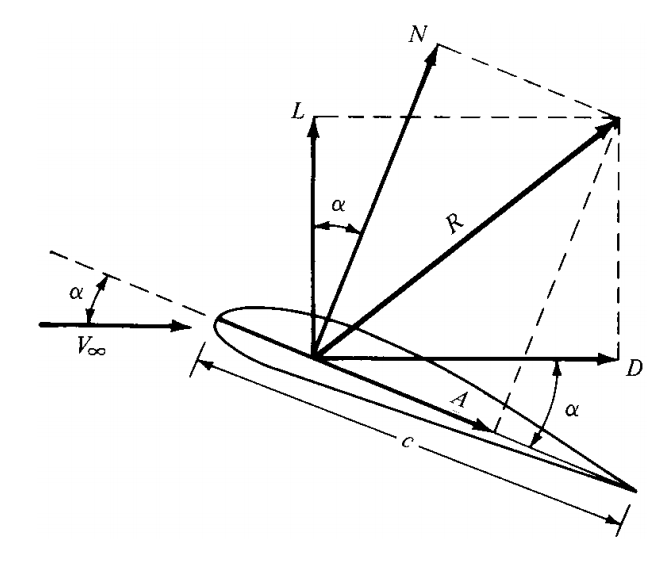
\includegraphics[width=.8\linewidth]{figuras/outras/anderson_profile_forces.png}
    \caption{Forças de arrasto (D) e sustentação (L) geradas em um corpo sujeito a um escoamento com velocidade de fluxo livre $V_{\infty}$, sob um angulo de ataque $\alpha$. Fonte: \cite{anderson1984fundamentals}}
    \label{fig:aero_profile_forces}
\end{figure}

\begin{figure}[H]
    \centering
    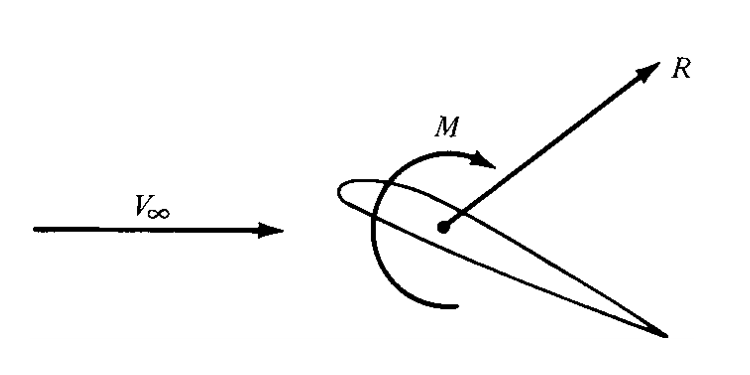
\includegraphics[width=.8\linewidth]{figuras/outras/anderson_profile_momentum.png}
    \caption{Momento (M) gerado em um corpo imerso em um escoamento com velocidade $V_{\infty}$. Fonte: \cite{anderson1984fundamentals}}
    \label{fig:aero_profile_momentum}
\end{figure}

Tomando-se uma área e um comprimento de referência (ambos arbitrados) pode-se expressar estas forças e momentos através de coeficientes adimensionais  \citep{anderson1984fundamentals}. Para o caso do momento, o mesmo é medido usualmente (em superfícies sustentadoras) ao redor do ponto a um quarto de corda, devido ao fato de que, quando medido neste ponto, o coeficiente apresenta relativa invariância com o ângulo de ataque ($\alpha$) \citep{abbott1959theory}. 

\begin{equation}
    C_L =  \frac{L}{ \frac{1}{2} \rho V_{\infty}^{2} S}
\end{equation}

\begin{equation} 
    C_D =  \frac{D}{ \frac{1}{2} \rho V_{\infty}^{2} S}
\end{equation}

\begin{equation}
    C_M =  \frac{M}{ \frac{1}{2} \rho V_{\infty}^{2} S C_{M.A.}}
\end{equation}

onde $L$ representa a força de sustentação, $D$ a força de arrasto, $M$ o momento, $\rho$ a densidade do ar, $V_{\infty}$ a velocidade de fluxo livre, $S$ a área de referencia e $C_{M.A.}$ a corda média aerodinâmica da geometria de referência.

A vantagem em se utilizar estes coeficientes se da pela relativa invariância dos mesmos para pequenas faixas de número de Reynolds, o que permite que, uma vez conhecidos os coeficientes, possam ser calculadas as forças e momento aerodinâmicos apenas conhecendo-se as características do escoamento \citep{anderson1984fundamentals}.

\begin{figure}[H]
    \centering
    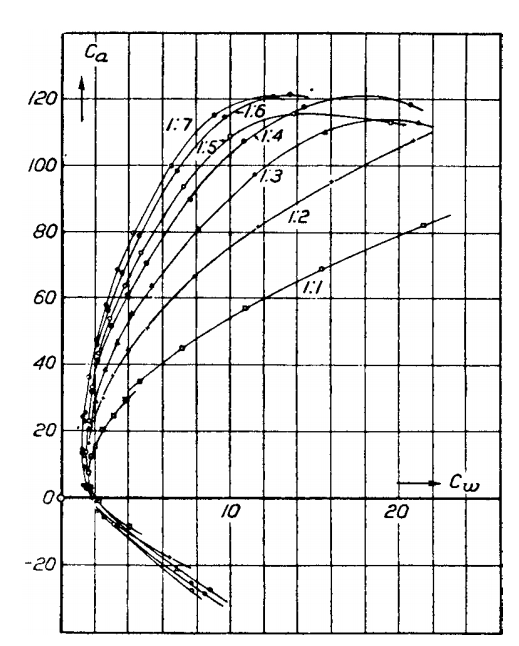
\includegraphics[width=.8\linewidth]{figuras/outras/drag_polar_prandtl.png}
    \caption{Exemplos de Polar de Arrasto para asas de diversas relações de envergadura sobre corda, em uma determinada faixa de Reynolds. O eixo das ordenadas representa $C_L$ e o eixo das abscissas $C_D$, ambos escalados por um fator de 100. Fonte: \cite{prandtl1921applications}}
    \label{fig:drag_polar_prandtl}
\end{figure}

É comum a apresentação gráfica dos coeficientes de sustentação em contraposição aos coeficientes em um mesmo gráfico (ver figura \ref{fig:drag_polar_prandtl}), para diferentes ângulos de ataque. Este gráfico é chamado Polar de Arrasto, e é uma representação gráfica do comportamento aerodinâmico de um corpo para uma determinada faixa de Reynolds \citep{prandtl1921applications}.

\section{Substituição do túnel de vento por bancada experimental}

Durante os estudos para desenvolvimento da aeronave X-57, no âmbito do projeto LEAPtech, \cite{murray2016leaptech} desenvolveram uma bancada de testes com funcionamento semelhante a da proposta neste trabalho. A bancada partiu da filosofia "all-up testing", proposta por George Mueller (NASA's Apollo) onde se reconhece a necessidade do teste integrado de sistemas (em oposição à realização somente de testes de sistemas isolados). Esta filosofia defende que em testes isolados o projetista procura por modos de falha conhecidos, enquanto em testes integrados o projetista busca a identificação de modos de falha desconhecidos, justamente pela dificuldade em se prever o comportamento dos sistemas quando não mais isolados. 

\begin{figure}[!ht]
    \centering
    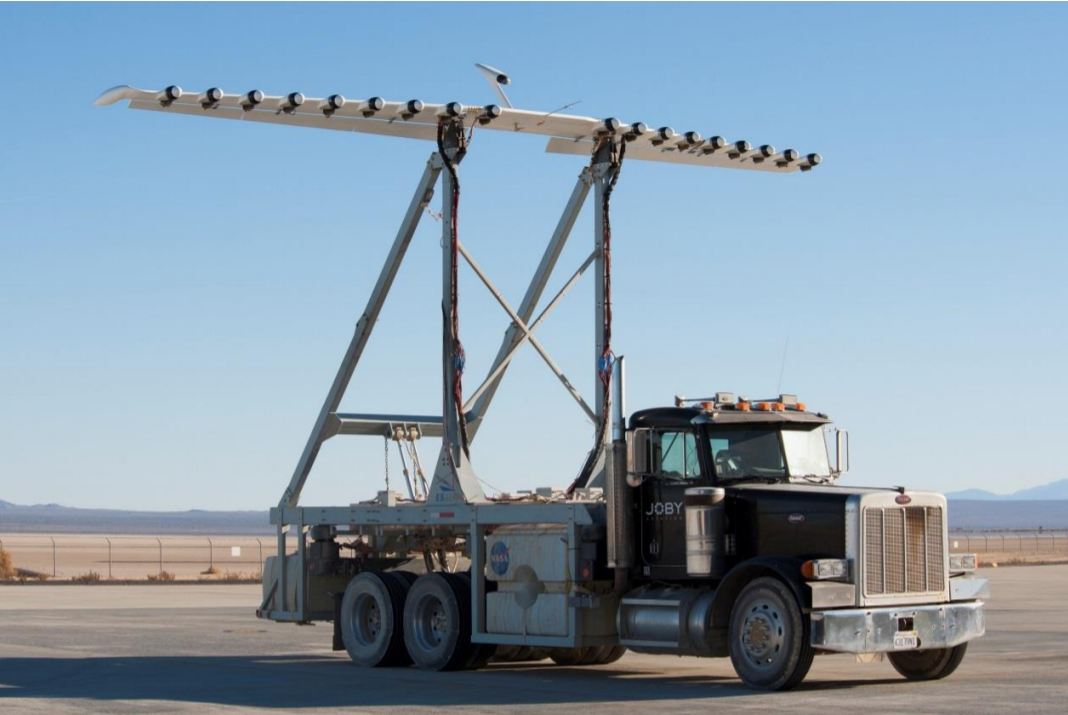
\includegraphics[width=.8\linewidth]{figuras/leaptech/leaptech1.png}
    \caption{Bancada experimental desenvolvida no âmbito do projeto LEAPTech. Fonte: \cite{murray2016leaptech}}
    \label{fig:leaptech1}
\end{figure}

A proposta de construção desta bancada (frente ao uso de um túnel de vento) se deu devido à necessidade de se realizar iterações no projeto (e, consequentemente, testes) com maior agilidade, devido à natureza inovativa do projeto (propulsão elétrica distribuída ao longo da asa com beneficiamento por ganho local de velocidade).

\begin{figure}[H]
    \centering
    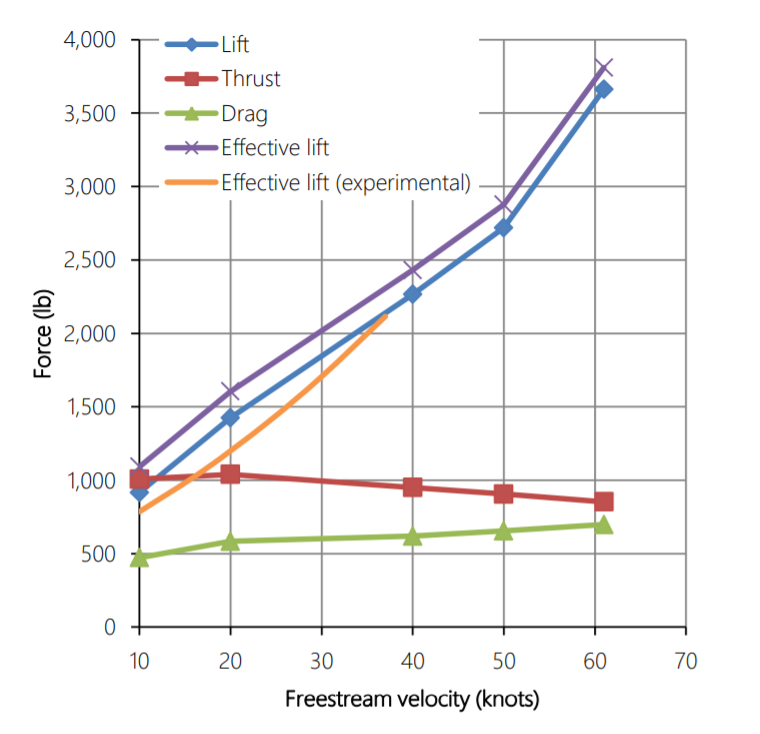
\includegraphics[width=.8\linewidth]{figuras/leaptech/cfd_comp.png}
    \caption{Comparações entre resultados de simulação CFD e dados experimentais no âmbito do projeto LEAPTech. Fonte: \cite{stoll2015comparison}}
    \label{fig:leaptech1}
\end{figure}

\cite{stoll2015comparison} realizou simulação CFD da asa da aeronave X-57 (com inclusão das hélices e seus efeitos) nos softwares STAR-CCM+ (RANS), FUN3D (RANS) e VSPAERO (VLM), e comparou os mesmos com os resultados obtidos na bancada desenvolvida. Foram encontradas diferenças menores que 10\% entre os resultados de simulação e os experimentais, indicando uma grande possibilidade deste método experimental ser valido para as avaliações desejadas.

\section{Considerações para o projeto da bancada}

\cite{gonzalez2011components} definem como principais pontos de atenção no projeto de uma balança para medição de forças aerodinâmicas os seguintes:

\begin{itemize}
    \item Calibração das células de carga individualmente - De acordo com os autores é necessário conhecer as incertezas de cada sensor individualmente para poder-se avaliar corretamente os efeitos de acoplamento. 
    \item Calibração da balança integrada - Mesmo com o conhecimento da incerteza das células individualmente, efeitos de acoplamento ocorrem nas medições, como resultado principalmente das deformações elásticas que ocorrem na estrutura da balança.
    \item Calibração para os efeitos dinâmicos - \cite{gonzalez2011components} ilustra valores típicos de carga na balança e vibrações induzidas pelo escoamento, mostrando que a ordem de grandeza da amplitude das cargas devido às vibrações pode ser a mesma da carga, comprometendo as medições.
    \item Avaliação da taxa de aquisição miníma dos sensores - No mesmo artigo é ilustrada a avaliação da taxa de amostragem dos dados de força através da sua média, mostrando que a média sofre uma oscilação para baixas taxas de aquisição até se estabilizar a partir de uma certa taxa de amostragem. Este mecanismo de avaliação pode ser utilizado em dados já adquiridos através da sub-amostragem dos dados.
    \item Filtragem dos dados - Segundo os autores, dado que as cargas devem ser invariantes no tempo para a situação estática, toma-se como aceitável a filtragem dos dados através de um filtro de médias-moveis.
\end{itemize}

\begin{figure}[!ht]
    \centering
    \caption{Exemplos de analises levantadas para garantir a qualidade dos dados medidos. Fonte: \cite{gonzalez2011components}}
        \subfloat[Demonstração de convergência do valor médio com o aumento da frequência de aquisição do dado.]{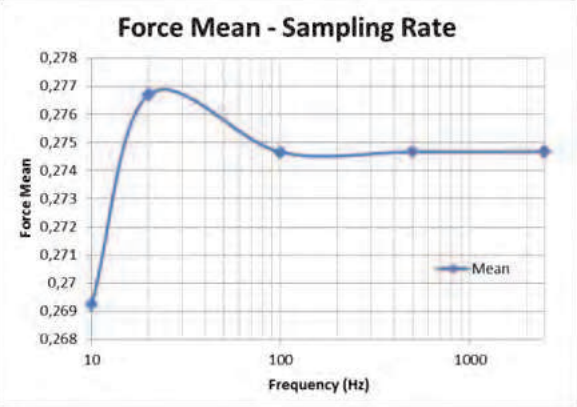
\includegraphics[width=0.4\columnwidth]{figuras/outras/convergence_rate.png}
        \label{convergence_rate}}
        \qquad
        \subfloat[Curva mostrando o acoplamento (indesejado) entre as forças de sustentação (L) e de arrasto (D), isto é, a falsa leitura de arrasto pelo sistema quando apenas a força de sustentação está presente.]{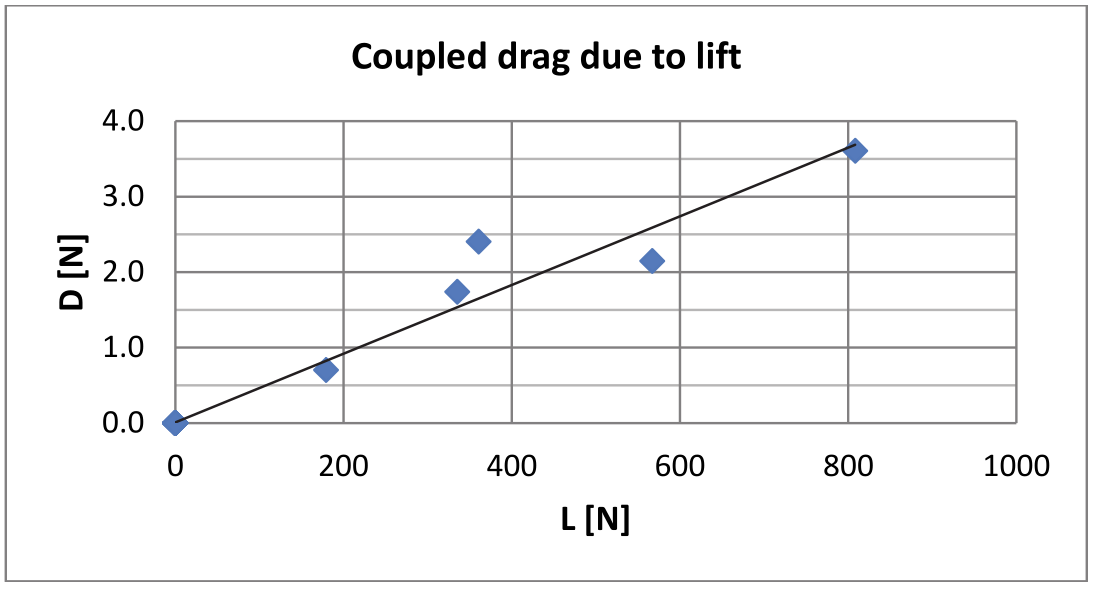
\includegraphics[width=0.4\columnwidth]{figuras/outras/coupled_forces.png}}
        \label{coupled_forces}
\end{figure}

As calibrações e análises estipuladas nos itens anteriores serão desenvolvidas ao longo deste trabalho.

% \section{Considerações quanto ao processamento dos dados gerados experimentalmente}
